\documentclass[
%DIF LATEXDIFF DIFFERENCE FILE
%DIF DEL /tmp/GlqwK9bk5O/latexdiff-vc-HEAD~1/thesis.tex   Wed Dec  9 07:53:23 2020
%DIF ADD thesis.tex                                       Wed Dec  9 08:08:31 2020
  ams,
  uplatex]{U-AizuGT}

\usepackage{pifont}
\usepackage{cite}
\usepackage[dvipdfmx]{graphicx}
\usepackage[dvipdfmx]{hyperref}

% ハイフネーション禁止
\hyphenpenalty=10000\relax
\exhyphenpenalty=10000\relax
\sloppy


% ここまで


\title{Writing a Thesis Using Markdown}
\author{Sachiko Tajima}
\studentid{s1250117}
\supervisor{Prof. Yutaka Watanobe}
\makeatletter
\@ifpackageloaded{subfig}{}{\usepackage{subfig}}
\@ifpackageloaded{caption}{}{\usepackage{caption}}
\captionsetup[subfloat]{margin=0.5em}
\AtBeginDocument{%
\renewcommand*\figurename{Figure}
\renewcommand*\tablename{Table}
}
\AtBeginDocument{%
\renewcommand*\listfigurename{List of Figures}
\renewcommand*\listtablename{List of Tables}
}
\@ifpackageloaded{float}{}{\usepackage{float}}
\floatstyle{ruled}
\@ifundefined{c@chapter}{\newfloat{codelisting}{h}{lop}}{\newfloat{codelisting}{h}{lop}[chapter]}
\floatname{codelisting}{Code}
\newcommand*\listoflistings{\listof{codelisting}{List of Listings}}
\makeatother

\bibliographystyle{ieicetr}
%DIF PREAMBLE EXTENSION ADDED BY LATEXDIFF
%DIF UNDERLINE PREAMBLE %DIF PREAMBLE
\RequirePackage[normalem]{ulem} %DIF PREAMBLE
\RequirePackage{color}\definecolor{RED}{rgb}{1,0,0}\definecolor{BLUE}{rgb}{0,0,1} %DIF PREAMBLE
\providecommand{\DIFaddtex}[1]{{\protect\color{blue}\uwave{#1}}} %DIF PREAMBLE
\providecommand{\DIFdeltex}[1]{{\protect\color{red}\sout{#1}}}                      %DIF PREAMBLE
%DIF SAFE PREAMBLE %DIF PREAMBLE
\providecommand{\DIFaddbegin}{} %DIF PREAMBLE
\providecommand{\DIFaddend}{} %DIF PREAMBLE
\providecommand{\DIFdelbegin}{} %DIF PREAMBLE
\providecommand{\DIFdelend}{} %DIF PREAMBLE
\providecommand{\DIFmodbegin}{} %DIF PREAMBLE
\providecommand{\DIFmodend}{} %DIF PREAMBLE
%DIF FLOATSAFE PREAMBLE %DIF PREAMBLE
\providecommand{\DIFaddFL}[1]{\DIFadd{#1}} %DIF PREAMBLE
\providecommand{\DIFdelFL}[1]{\DIFdel{#1}} %DIF PREAMBLE
\providecommand{\DIFaddbeginFL}{} %DIF PREAMBLE
\providecommand{\DIFaddendFL}{} %DIF PREAMBLE
\providecommand{\DIFdelbeginFL}{} %DIF PREAMBLE
\providecommand{\DIFdelendFL}{} %DIF PREAMBLE
%DIF HYPERREF PREAMBLE %DIF PREAMBLE
\providecommand{\DIFadd}[1]{\texorpdfstring{\DIFaddtex{#1}}{#1}} %DIF PREAMBLE
\providecommand{\DIFdel}[1]{\texorpdfstring{\DIFdeltex{#1}}{}} %DIF PREAMBLE
\newcommand{\DIFscaledelfig}{0.5}
%DIF HIGHLIGHTGRAPHICS PREAMBLE %DIF PREAMBLE
\RequirePackage{settobox} %DIF PREAMBLE
\RequirePackage{letltxmacro} %DIF PREAMBLE
\newsavebox{\DIFdelgraphicsbox} %DIF PREAMBLE
\newlength{\DIFdelgraphicswidth} %DIF PREAMBLE
\newlength{\DIFdelgraphicsheight} %DIF PREAMBLE
% store original definition of \includegraphics %DIF PREAMBLE
\LetLtxMacro{\DIFOincludegraphics}{\includegraphics} %DIF PREAMBLE
\newcommand{\DIFaddincludegraphics}[2][]{{\color{blue}\fbox{\DIFOincludegraphics[#1]{#2}}}} %DIF PREAMBLE
\newcommand{\DIFdelincludegraphics}[2][]{% %DIF PREAMBLE
\sbox{\DIFdelgraphicsbox}{\DIFOincludegraphics[#1]{#2}}% %DIF PREAMBLE
\settoboxwidth{\DIFdelgraphicswidth}{\DIFdelgraphicsbox} %DIF PREAMBLE
\settoboxtotalheight{\DIFdelgraphicsheight}{\DIFdelgraphicsbox} %DIF PREAMBLE
\scalebox{\DIFscaledelfig}{% %DIF PREAMBLE
\parbox[b]{\DIFdelgraphicswidth}{\usebox{\DIFdelgraphicsbox}\\[-\baselineskip] \rule{\DIFdelgraphicswidth}{0em}}\llap{\resizebox{\DIFdelgraphicswidth}{\DIFdelgraphicsheight}{% %DIF PREAMBLE
\setlength{\unitlength}{\DIFdelgraphicswidth}% %DIF PREAMBLE
\begin{picture}(1,1)% %DIF PREAMBLE
\thicklines\linethickness{2pt} %DIF PREAMBLE
{\color[rgb]{1,0,0}\put(0,0){\framebox(1,1){}}}% %DIF PREAMBLE
{\color[rgb]{1,0,0}\put(0,0){\line( 1,1){1}}}% %DIF PREAMBLE
{\color[rgb]{1,0,0}\put(0,1){\line(1,-1){1}}}% %DIF PREAMBLE
\end{picture}% %DIF PREAMBLE
}\hspace*{3pt}}} %DIF PREAMBLE
} %DIF PREAMBLE
\LetLtxMacro{\DIFOaddbegin}{\DIFaddbegin} %DIF PREAMBLE
\LetLtxMacro{\DIFOaddend}{\DIFaddend} %DIF PREAMBLE
\LetLtxMacro{\DIFOdelbegin}{\DIFdelbegin} %DIF PREAMBLE
\LetLtxMacro{\DIFOdelend}{\DIFdelend} %DIF PREAMBLE
\DeclareRobustCommand{\DIFaddbegin}{\DIFOaddbegin \let\includegraphics\DIFaddincludegraphics} %DIF PREAMBLE
\DeclareRobustCommand{\DIFaddend}{\DIFOaddend \let\includegraphics\DIFOincludegraphics} %DIF PREAMBLE
\DeclareRobustCommand{\DIFdelbegin}{\DIFOdelbegin \let\includegraphics\DIFdelincludegraphics} %DIF PREAMBLE
\DeclareRobustCommand{\DIFdelend}{\DIFOaddend \let\includegraphics\DIFOincludegraphics} %DIF PREAMBLE
\LetLtxMacro{\DIFOaddbeginFL}{\DIFaddbeginFL} %DIF PREAMBLE
\LetLtxMacro{\DIFOaddendFL}{\DIFaddendFL} %DIF PREAMBLE
\LetLtxMacro{\DIFOdelbeginFL}{\DIFdelbeginFL} %DIF PREAMBLE
\LetLtxMacro{\DIFOdelendFL}{\DIFdelendFL} %DIF PREAMBLE
\DeclareRobustCommand{\DIFaddbeginFL}{\DIFOaddbeginFL \let\includegraphics\DIFaddincludegraphics} %DIF PREAMBLE
\DeclareRobustCommand{\DIFaddendFL}{\DIFOaddendFL \let\includegraphics\DIFOincludegraphics} %DIF PREAMBLE
\DeclareRobustCommand{\DIFdelbeginFL}{\DIFOdelbeginFL \let\includegraphics\DIFdelincludegraphics} %DIF PREAMBLE
\DeclareRobustCommand{\DIFdelendFL}{\DIFOaddendFL \let\includegraphics\DIFOincludegraphics} %DIF PREAMBLE
%DIF LISTINGS PREAMBLE %DIF PREAMBLE
\RequirePackage{listings} %DIF PREAMBLE
\RequirePackage{color} %DIF PREAMBLE
\lstdefinelanguage{DIFcode}{ %DIF PREAMBLE
%DIF DIFCODE_UNDERLINE %DIF PREAMBLE
  moredelim=[il][\color{red}\sout]{\%DIF\ <\ }, %DIF PREAMBLE
  moredelim=[il][\color{blue}\uwave]{\%DIF\ >\ } %DIF PREAMBLE
} %DIF PREAMBLE
\lstdefinestyle{DIFverbatimstyle}{ %DIF PREAMBLE
	language=DIFcode, %DIF PREAMBLE
	basicstyle=\ttfamily, %DIF PREAMBLE
	columns=fullflexible, %DIF PREAMBLE
	keepspaces=true %DIF PREAMBLE
} %DIF PREAMBLE
\lstnewenvironment{DIFverbatim}{\lstset{style=DIFverbatimstyle}}{} %DIF PREAMBLE
\lstnewenvironment{DIFverbatim*}{\lstset{style=DIFverbatimstyle,showspaces=true}}{} %DIF PREAMBLE
%DIF END PREAMBLE EXTENSION ADDED BY LATEXDIFF

\begin{document}
    \maketitle

    \hypertarget{abstract}{%
    \section{Abstract}\label{abstract}}

    This is a template writtten is a Markdown following the University of
    Aizu graduation thesis format \cite{graduation-thesis}. If you have any
    quessstions or something you don't understand, just refer to
    kuee-thesis-markdown \cite{kuee-thesis-markdown} .

    \hypertarget{introduction}{%
    \section{Introduction}\label{introduction}}

    If you want to put figure or graph in thesis, write in the text as in
    \LaTeX writing.

    The \LaTeX Distribution kit includes the following files in table
    \ref{tab:kit} .

    \begin{table}[htbp]
      \caption{The kit distribution}\label{tab:kit}
      \begin{center}
        \begin{tabular}{ll}
          \verb+U-AizuGT.cls+ &  \LaTeX2e{} 's document classfile       \\
          \verb+ieicetr.bst+ & document style file \cite{ieicetr} \\
          \verb+thesis.bib+ & references file              \\
        \end{tabular}
      \end{center}
    \end{table}

    \hypertarget{reference}{%
    \subsection{Reference}\label{reference}}

    Nara suteki daigaku \cite{nara-nice} tekina.

    \hypertarget{table}{%
    \subsection{Table}\label{table}}

    aiueo kakikukeko sashisuseso tatituteto naninuneno hahihuheho mamimumemo
    yayuyo rarirurero wawon.

    \begin{table}[htbp]
      \caption{Sample of Figure $\cdot$ Table}\label{tab:fig}
      \begin{center}
        \begin{tabular}{|l|r|}
          \hline
          \verb+\textwidth+ & 424pt + 1cm  \\ \hline
          \verb+\textheight+ & 604pt + 67pt \\ \hline
          \verb+\oddsidemargin+ & 0pt          \\ \hline
          \verb+\evensidemargin+ & 0pt          \\ \hline
          \verb+\topmargin+ & 0pt          \\ \hline
          \verb+\headheight+ & 0pt          \\ \hline
          \verb+\headsep+ & 0pt          \\ \hline
          \verb+\footskip+ & 0pt          \\ \hline
        \end{tabular}
      \end{center}
    \end{table}

    \hypertarget{figure}{%
    \subsection{Figure}\label{figure}}

    \begin{figure}[htbp]
      \centering
      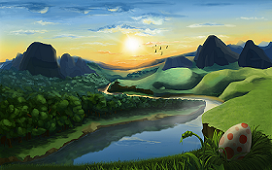
\includegraphics[scale = 1.0]{image.png}
      \caption{hogehoge}\label{fig:hogehoge}
    \end{figure}

    \hypertarget{material-methods}{%
    \section{Material \& Methods}\label{material-methods}}

    text tessssx ttexte

    \hypertarget{results}{%
    \section{Results}\label{results}}

    t e x t t e s s ss x t t exte

    \hypertarget{conclusion}{%
    \section{Conclusion}\label{conclusion}}

    text tes sssx tt exte

    \hypertarget{bobliography}{%
    \section{Bobliography}\label{bobliography}}

    text tess ssxt text e

    \hypertarget{acknowledgements}{%
    \section{Acknowledgements}\label{acknowledgements}}

    texttessssxttexte

        \bibliography{thesis.bib}


\end{document}
